\documentclass[UTF8,a4paper,10pt]{ctexart}
\usepackage[margin=19mm,top=20mm,bottom=19mm]{geometry}
\usepackage{amsmath,amssymb,booktabs,tabularx,graphicx,xcolor,fancyhdr,enumitem,tikz}
\usetikzlibrary{arrows.meta,positioning}
\usepackage[colorlinks=true,linkcolor=teal,urlcolor=teal]{hyperref}
\definecolor{ink}{HTML}{142B43}\definecolor{accent}{HTML}{168579}
\pagestyle{fancy}\fancyhf{}\fancyhead[L]{\small CF2026 Project 1}\fancyhead[R]{\small 青序量化研究平台}
\fancyfoot[L]{\scriptsize 研究版本 V3 / 2026-09-22 · 固定历史快照 · 描述性结果}\fancyfoot[R]{\thepage/10}
\setlength{\headheight}{14pt}\setlength{\parskip}{4pt}\setlength{\emergencystretch}{2em}\setlength{\parindent}{2em}
\setlist{nosep,leftmargin=1.7em}\ctexset{section={format=\Large\bfseries\color{ink}},subsection={format=\normalsize\bfseries\color{accent}}}
\newcommand{\lead}[1]{\noindent{\bfseries\color{accent}#1}\par}
\newcommand{\page}[1]{\newpage\section*{#1}}
\begin{document}
\begin{center}{\small\color{accent}COMPUTATIONAL FINANCE / PROJECT 1}\\[8pt]
{\Huge\bfseries\color{ink}青序量化研究平台}\\[8pt]
{\Large 指数目标、滚动预测与策略版本管理}\\[8pt]
2026年9月22日\quad V3研究更新\quad 最终提交报告
\end{center}
\section*{1\quad 目标与主要结果}
\lead{从购买力目标升级为扣费后超过沪深300，同时保留选择失败与全部候选。}
平台覆盖数据质量、因子、横截面诊断、含费用回测、独立账本和可复现交付。用户将策略目标改为战胜沪深300。本轮固定1,000股历史池及2025-01-02至2026-09-18区间，预先限定8个候选，比较经济主题、年度滚动Ridge、年度滚动LightGBM及固定融合。

当前默认策略为\textbf{年度滚动LightGBM＋波动预算}，用24个标准化/中性化输入预测股票相对排序，50只目标持仓，每20个交易日调仓，允许现金、不用杠杆。
\begin{center}\begin{tabular}{lr}\toprule
2025--2026固定417日历史区间 & 结果\\\midrule
累计净收益 / 年化净收益 & 25.13\% / 14.51\%\\
最大回撤 / 年化Sharpe & 9.88\% / 1.255\\
沪深300价格指数 / 全收益指数 & 14.55\% / 19.94\%\\
超过价格指数 / 全收益指数 & 10.58 / 5.19个百分点\\
交易费用 / 平均现金 & 24,506.76元 / 17.87\%\\\bottomrule
\end{tabular}\end{center}
\textbf{本段历史同时超过价格指数和含红利再投资的全收益指数。}双倍交易费用仍收益22.48\%，信号延后一日收益27.31\%。2023起连续运行累计44.09\%、最大回撤19.70\%，但2024年度落后价格指数7.28个百分点，不能声称每年都战胜市场。

\subsection*{选择边界必须与结果一起阅读}
V3验证期预选的价值质量组合在2025--2026仅收益4.30\%，没有超过指数。当前LightGBM是在查看本轮历史结果后，从通过验证净收益、超额收益和回撤门槛的候选中选出。V2已经看过同一最终区间，本次\textbf{不是独立盲测成功}。保留失败预选和8个候选，下一步应冻结规则做新数据前向验证。
\subsection*{交付与操作}
“回测实验”现在可切换V1单因子、V2各模型和V3候选，默认最新历史验收达标版本。账本正确与收益/风险验收分开；亏损或回撤超门槛显示未达标。报告、20页Beamer、可编辑PPTX和讲稿与平台使用同一派生证据。
\page{2\quad 架构、接口与可维护性}
\lead{数据、分数、目标权重、成交和统计分别承担独立职责。}
选择Python，复用NumPy、pandas、SciPy、scikit-learn及LightGBM。Streamlit和Plotly负责交互；界面不实现第二套收益计算。参考Qlib的因子表达与训练/验证工作流，保留透明的小型会计引擎，以便逐项核对课程的缺失、费用和标签口径。Backtrader仅作为独立参考测试依赖。
\begin{center}\begin{tikzpicture}[node distance=5mm and 5mm, every node/.style={draw=ink,rounded corners,align=center,font=\small,minimum height=9mm},>=Stealth]
\node(a){原始快照\\质量与哈希};\node[right=of a](b){因子/模型\\日期×资产分数};\node[right=of b](c){组合构建\\目标权重＋现金};\node[right=of c](d){成交账本\\成交/持仓/净值};
\draw[->](a)--(b);\draw[->](b)--(c);\draw[->](c)--(d);
\node[below=of c](e){诊断、实验记录与中文界面};\draw[->](b)|-(e);\draw[->](d)|-(e);
\end{tikzpicture}\end{center}
\noindent\begin{tabularx}{\textwidth}{lX}\toprule
模块 & 输入、输出与职责\\\midrule
data / incremental & 厂商响应转统一行情；原始响应与标准数据分开，重复键报错，增量合并另写新目录。\\
factors / features & 三个注册式基准因子及12个扩展因子；完整日历对齐，输出长表或日期×资产面板。\\
models & 只对训练区间拟合，输出后续分数与固定参数、随机种子。\\
risk / portfolio & 分数变为目标权重；保留缓冲、波动率预算及行业/单股上限。\\
engine & 下一开盘执行、现金约束、涨跌停、部分成交、缺失估值及逐日账本。\\
analytics & IC、分组、收益与回撤；独立从成交重建现金和单位余额。\\
experiment / research & 配置、数据和源码哈希，固定对照、时间分割、选择记录、历史运行归档。\\
app / strategies / UI & 调用核心或读取已落盘研究结果，导出CSV/PDF，不在刷新时偷偷重训。\\\bottomrule
\end{tabularx}
\subsection*{核心数据契约}
行情键为\texttt{date, asset}；因子长表为\texttt{date, asset, factor, value}，高分方向在实验前固定。目标权重保留同样日期和资产轴，要求有限、非负且和不超过1。成交结果分为daily、trades、positions、orders，拒单原因和部分成交均留痕。CLI与界面使用同一配置与函数。
\subsection*{扩展路径与版本}
新增技术因子注册FactorSpec；基本面因子显式声明公告滞后；预测模型只输出相同面板。新组合只替换权重构建，成交与分析无需改写。完整研究重跑前归档旧目录；特征缓存核对输入文件及源码指纹，避免把旧特征冒充新版本。公开仓库不包含Token或厂商逐股原始数据。

版本目录独立记录信号、组合规则、分数来源和状态；切换版本即清除旧结果。参数重跑沿用同一成交核心，每次另存运行目录。仅公开聚合日账本，逐股财务和模型缓存保留在本地。
\page{3\quad 数据来源、质量与偏差}
\lead{固定选池日先于所有收益研究，历史缺失保留并计数。}
2019-12-31按当日成交额取符合主板代码、价格至少3元且有成交的前1,000只，并列按代码。没有使用今日仍上市名单，后来停止报价的原成员也保留。该池不包括2020年以后IPO，单日流动性选择偏向当时热点，结论不代表全A股或沪深300。
\begin{center}\begin{tabular}{lr}\toprule
核验项目 & 数量或结果\\\midrule
统一日线 / 日历交易日 & 1,656,599 / 1,690\\
完整股票×日历网格缺行 & 33,401\\
重复行情键 / 异常剔除 & 0 / 0\\
涨跌停价格缺失 / 最新有报价资产 & 48 / 956\\
每日估值记录 / 重复键 & 1,656,599 / 0\\
财务指标记录 / 单次返回最高行数 & 57,389 / 67（接口上限100）\\
行业历史区间 / 特征网格 & 1,432 / 1,690,000\\
原行情清单哈希 / 新研究清单哈希 & 3,006 / 2,073个文件通过\\\bottomrule
\end{tabular}\end{center}
\noindent\begin{tabularx}{\textwidth}{lX}\toprule
来源接口 & 字段、单位与用途\\\midrule
daily / adj\_factor & OHLC原价为元/股，vol源单位手转股；统一乘法复权供收益计算。\\
stk\_limit / trade\_cal & 原始涨跌停价和完整交易日历；缺限制价时不执行对应方向。\\
daily\_basic & total\_mv为万元，PE/PB为倍数，dv\_ttm与换手率为百分数；每日横截面。\\
fina\_indicator & ann\_date为公告日，end\_date为报告期；ROE为百分数，严格滞后使用。\\
index\_member\_all & 申万一级行业进出区间；未知或冲突标UNKNOWN，不将当前行业反填历史。\\
index\_daily / cn\_cpi & 沪深300价格/全收益指数；全国CPI月环比，按共同完整月份比较。\\\bottomrule
\end{tabularx}
\subsection*{复权、可得性与存储}
所有OHLC用\(P^{adj}_{i,t}=P^{raw}_{i,t}A_{i,t}/A_{i,ref}\)，每资产固定首个有效参考因子。原行情及V2研究缓存合计约1.63GB，包括原始缓存、标准数据、特征和模型分数。原始请求记录字段、日期与UTC下载时间，保存SHA-256；同请求可断点续拉。

历史行业未知比例约0.52\%，年度ROE平均覆盖约98.90\%（按每日合资格样本计算）。采用公告时点仍不能消除厂商事后修订，当前数据不是完整的逐版本财报库。保留此局限，不用“无未来函数”概括所有数据风险。

新增基准由Tushare指数目录确认H00300.CSI，再取全收益日线；另取510330.SH基金日线和复权因子，各1,690日。价格指数、全收益指数、ETF代理分开命名，未猜测或替代指数代码。
\page{4\quad 因子设计与标准接口}
\lead{12个因子覆盖不同假设，经济方向固定，负结果同样保留。}
记\(C,H,L,V\)为同尺度价格与股数，\(r_t=C_t/C_{t-1}-1\)。下表所有分数均为“越大越优先”的事前方向，缺失不补未来值。完整字段、窗口、失败情形和实现位置见\texttt{docs/FACTOR\_CARDS\_V2.md}。
\begin{center}\small\begin{tabular}{lll}\toprule
因子 & 公式与窗口 & 主要假设或风险\\\midrule
中期动量 & \(C_{t-20}/C_{t-60}-1\) & 跳过短期反转；趋势突变失效\\
短期反转 & \(-(C_t/C_{t-5}-1)\) & 超调修复；持续下跌失效\\
低波动 & \(-s(r,20)\) & 防御性；牛市可能落后\\
低振幅 & \(-\overline{(H-L)/C}_{20}\) & 日内风险；与低波动冗余\\
均线趋势 & \(C_t/\overline C_{20}-1\) & 趋势延续；震荡易反复\\
量能变化 & \(\log(\overline V_5/\overline V_{20})\) & 量能确认；方向可能不稳定\\
流动性 & \(-\overline{|r|/(C^{raw}V/10^6)}_{20}\) & 冲击较低；可能偏大盘\\
低换手 & \(-turnover\_rate\) & 降低拥挤；也可能缺乏交易\\
盈利收益率 & \(1/PE_{TTM},\ PE>0\) & 价值；亏损公司无定义\\
账面市值比 & \(1/PB,\ PB>0\) & 价值；资产质量有差异\\
股息率 & \(dv_{TTM}/100\) & 分红；历史分红不可保证\\
盈利质量 & 最新已公告年度\(ROE/100\) & 盈利能力；财报修订与滞后\\\bottomrule
\end{tabular}\end{center}
动量和反转要求整个价格窗口完整，波动等滚动统计要求完整观测；不将停牌前后压缩为相邻日。PE/PB非正为缺失，财报同公告、同报告期的冲突副本剔除，年度报表超过550日不再使用。建模时至少10个有效因子；剩余标准化缺值填0表示当日横截面中性值，不将缺失收益标签填0。
\subsection*{基础项与扩展项的关系}
原始20日动量、5日反转、20日低波动保留注册入口，可独立调窗口、诊断和回测。12因子研究采用固定配方，标准化等权平均为一个透明基线。中性化改变行业/市值暴露，不保证提高收益；本次没有因为某因子最终IC为负而翻转符号。
\subsection*{与Qlib和参考论文的关系}
参考Qlib Alpha158中的滞后、滚动量价表达以及训练/验证分离，复用LightGBM和scikit-learn模型实现。此处12因子是明确列出的自定义子集，\textbf{未声称完整复制Alpha158，也未将Qlib引擎集成进主账本}。CogAlpha论文采用代码形式的因子与LLM演化搜索，本项目借鉴可检查的因子表示，未开展大规模自动搜索。

\page{5\quad 中性化、年度训练与8个候选}
\lead{因子处理按日进行；新模型只能使用当时已实现的标签。}
当日合资格因子按1\%/99\%截尾并用样本标准差标准化。对当日行业虚拟变量和对数市值回归取残差，再缩放为单位样本标准差。LightGBM同时输入12个标准化值和12个残差值，Ridge只输入12个残差值。
\[
z_{i,t}=\sum_g\alpha_{g,t}\mathbf1\{g_{i,t}=g\}+\beta_t\log MV_{i,t}+\epsilon_{i,t},\qquad n_{i,t}=\epsilon_{i,t}/s_t(\epsilon).
\]
每年第一次交易前一交易日形成新模型，训练此前3年。标签为次日开盘至20交易日后开盘收益的日横截面百分位减0.5，训练标签退出日必须严格早于模型形成日。整个下一年度使用该模型，到下一年才重训。
\begin{center}\small\begin{tabular}{lrr}\toprule
预测年度 & 训练观测数 & 最大标签退出日早于形成日\\\midrule
2023 & 654,563 & 已核验\\2024 & 645,816 & 已核验\\2025 & 636,902 & 已核验\\2026 & 634,716 & 已核验\\\bottomrule
\end{tabular}\end{center}
\begin{itemize}
\item 经济主题：价值（盈利/账面/股息）占50\%，ROE占25\%，低波动/低振幅占25\%。
\item Ridge：alpha=100，年度滚动重训，无最终期参数扫描。
\item LightGBM：250树，学习率0.03，15叶，最大深度5，最小叶500，L2=10，列采样0.8，种子20260921。
\item 固定融合：LightGBM百分位50\%、Ridge百分位25\%、经济主题百分位25\%。
\end{itemize}
四种信号各配稳定仓位及波动预算两种组合，共8个候选。稳定版本取消波动缩放和趋势折减；其他持仓、缓冲、上限及成交规则相同。2023--2024先记录验证结果及预选，然后再运行固定2025--2026区间。全部尝试保留在同一表。
\subsection*{与原建议的关系}
CNN需要有意义的局部邻接结构，简单排列的因子列没有天然邻接。V2已经保留小型MLP对照；本轮使用适合表格特征的树模型及线性基线，并未假定模型越复杂越好。年度训练减少长期冻结模型的陈旧性，但不能消除分布变化或过拟合。
\page{6\quad 组合、成交与账本核验}
\lead{每笔费用来自实际成交金额，模型只决定分数。}
每20个交易日调仓，目标50只。原持仓仍在前70名则优先保留，其余按分数补足，减少边界换手。先按波动率倒数构建权重，单股目标不超过4\%、行业目标不超过25\%；上限造成的余量留现金，不强制重新分配。

过去60日的候选组合收益估计年化波动率\(\hat\sigma\)。股票总预算为
\[
e_t=0.95\min\{1,0.20/\hat\sigma_t\}\times
\begin{cases}1,&CSI300_t\ge MA_{120,t},\\0.75,&\text{其他情况}.\end{cases}
\]
再应用个股与行业上限。所有估计截至形成日，次日开盘执行。风险估计中的少量历史缺价按0收益处理，是可低估风险的近似；实际缺价成交仍受阻。权重、波动和25\%回撤均为目标，不能保证市场变化后的实际风险。
\subsection*{成交与估值规则}
开盘按目标名义金额计算连续可分的复权单位，先卖后买，保留费用缓冲，现金不足同比缩减买单。涨停不买、跌停不卖、缺开盘或限制价不成交。每资产成交预算不超过此前20日平均成交额的1\%，超过时部分成交；这是事前容量代理，不是当日成交量的真实参与率保证。
\[
fee_t=0.001\,BuyNotional_t+0.0015\,SellNotional_t,\quad
Turnover_t=\frac{BuyNotional_t+SellNotional_t}{OpeningNAV_t}.
\]
买10bp、卖15bp是统一研究假设，不冒充历史法定税费。停牌持仓沿用最后已知收盘价并计数，连续缺失超过20个交易日保守计零；保留单位，恢复报价时重新估值，不虚构卖出。复权单位近似分红自动再投资，尚未模拟整手、完整分红现金或结算规则。
\subsection*{独立核验与扩展测试}
从成交逐笔重建现金与单位余额，再核对每日NAV、费用、换手与收益连乘。21个V3研究及压力运行全部通过，分别检查417、484或901个交易日。数值容差现金绝对\(10^{-6}\)元、相对\(10^{-10}\)。测试另覆盖手算、拆股连续性、独立Backtrader参考、未来扰动、公告滞后、中性化残差、无杠杆、部分成交及增量幂等。另以大面板逐项除法复现并修复本机可选NumExpr加速的错误常数结果，统一禁用该路径并重新生成全部研究；独立账本不能替代上游数值验证。最终测试与复算日志见验收清单。

\page{7\quad 失败、预选与开发后的候选}
\lead{更改研究目标不等于抹去原始失败。}
V1的20日动量、5日调仓长区间净收益为$-83.57\%$，最大回撤89.83\%；零费用独立重跑仍为$-75.16\%$。费用加回同成交路径得到$-58.12\%$，并非零费用独立策略，因为再投资路径不同。V2预选多因子在固定最终区间收益6.12\%，实现CPI目标但落后指数。
\subsection*{V3选择过程}
协议先写定8个候选与验证规则：2023--2024净收益、累计超额为正，最大回撤不超过25\%；先比较最差年度超额，再比较累计超额。价值质量主题稳定仓位排名第一，验证收益24.27\%、回撤9.16\%；但随后收益4.30\%，落后价格指数10.25个百分点。\textbf{这个预选失败不能被后续冠军替换。}
\begin{center}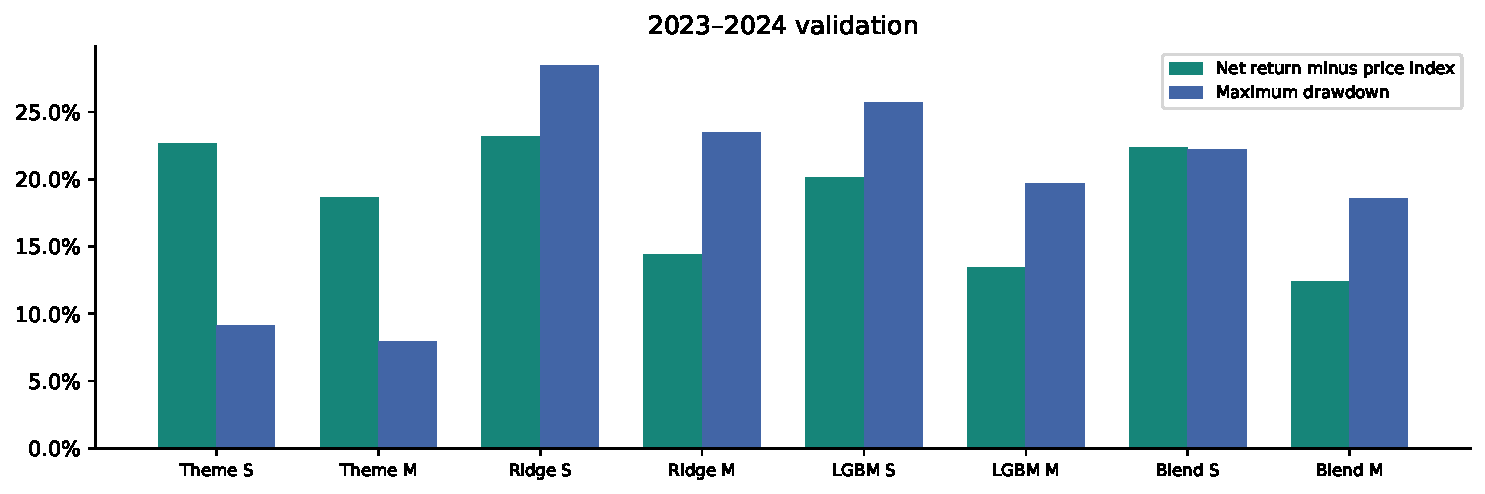
\includegraphics[width=.98\textwidth]{figures/validation.pdf}\end{center}
按用户要求进一步寻找能超过指数的历史候选，筛掉验证回撤超25\%的版本，再查看2025--2026超额。LightGBM稳定仓位虽然最终收益27.39\%，但验证回撤25.73\%，未作为默认。采用LightGBM波动预算版本，验证收益15.05\%、回撤19.70\%，最终收益25.13\%、回撤9.88\%。

以上是\textbf{开发后历史验收}，并非只有训练样本上的拟合收益，但也不属于全新盲测。决策文件保存preselected和selected两个字段，明确选择先后及8次候选规模。
\page{8\quad 固定区间的全候选与基准}
\lead{同一417日区间，策略费用已扣；基准名称及计息规则明确。}
\begin{center}\small\begin{tabular}{lrrr}\toprule
候选（稳定/波动预算） & 净收益 & 超价格指数 & 最大回撤\\\midrule
主题/稳定 & 4.30\% & -10.25\% & 9.13\%\\
主题/预算 & 5.68\% & -8.87\% & 8.76\%\\
Ridge/稳定 & 18.78\% & 4.23\% & 16.33\%\\
Ridge/预算 & 16.57\% & 2.02\% & 16.03\%\\
LGBM/稳定 & 27.39\% & 12.84\% & 9.75\%\\
LGBM/预算 & 25.13\% & 10.58\% & 9.88\%\\
融合/稳定 & 7.91\% & -6.64\% & 12.39\%\\
融合/预算 & 8.13\% & -6.42\% & 12.28\%\\\bottomrule\end{tabular}\end{center}
\begin{center}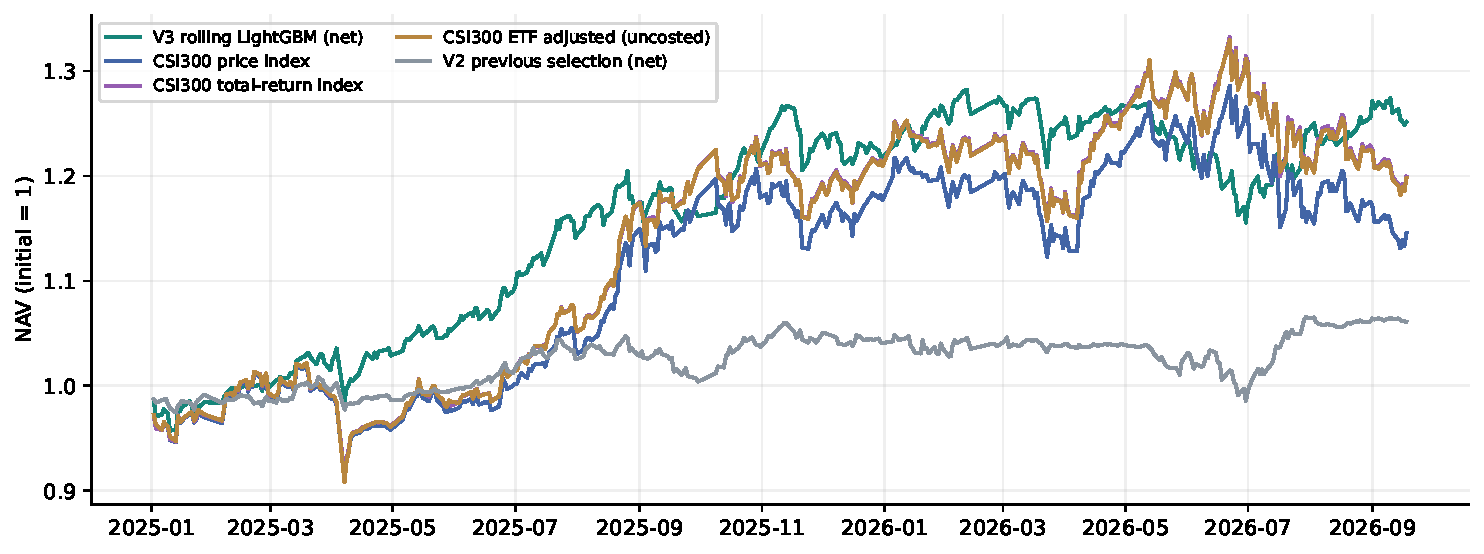
\includegraphics[width=.98\textwidth]{figures/nav.pdf}\end{center}
价格指数从前一交易日收盘归一化，累计14.55\%；全收益指数计红利再投资，累计19.94\%。策略同区间净收益25.13\%，相对全收益指数财富增长为$(1+25.13\%)/(1+19.94\%)-1\approx4.33\%$，与相差5.19个百分点是不同口径。

首次开盘起算价格指数收益14.64\%，结论不变。510330.SH复权未扣费代理收益19.82\%，另保留同开盘建仓扣买费的可交易近似；ETF不能改名为全收益指数。策略beta约0.30，年化跟踪误差15.60\%，信息比率0.292；落后阶段及主动净值回撤约18.41\%仍存在。
\page{9\quad 压力测试、诊断与长期区间}
\begin{center}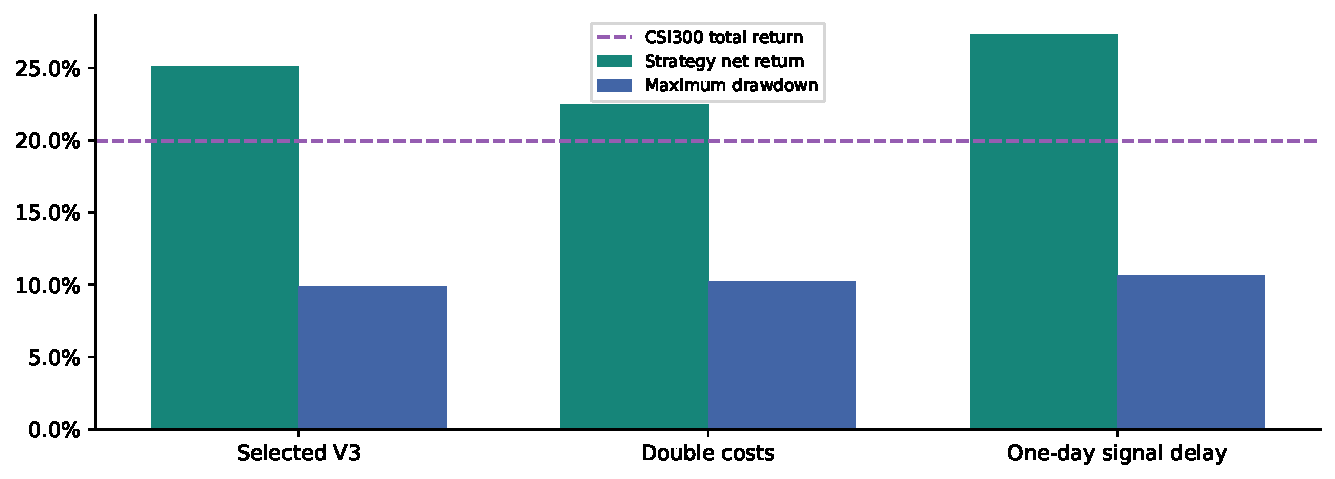
\includegraphics[width=.98\textwidth]{figures/controls.pdf}\end{center}
双倍费用重跑净收益22.48\%、回撤10.19\%；信号延后一交易日重跑净收益27.31\%、回撤10.67\%。两者仍超过同区间全收益指数19.94\%。延迟改善不是可再选择的默认参数，只是固定压力检查；没有据此改成更高收益的延迟版本。
\subsection*{从2023年连续运行，避免年度重置资金}
累计收益44.09\%，同期全收益指数28.86\%，策略最大回撤19.70\%。2023、2024、2025、2026年截至9月的净收益分别为7.12\%、7.41\%、22.44\%、2.28\%。2024落后价格指数7.28个百分点；长期优势不能解释为每年都赢。该连续账本与2025从现金起步的复核账本不同，年度收益不能互换。
\subsection*{课程因子诊断仍独立保留}
逐日计算Pearson IC和平均并列秩Spearman Rank IC，常数或不足有效样本返回缺失；不把股票日混为一次相关。先依据形成日分数分五组，再匹配未来标签，保留形成/有效人数；缺失标签不重新排名。878个形成日的12因子诊断保留在V2证据目录，低波动/低振幅平均Rank IC约0.072/0.079，流动性约$-0.051$，未因结果为负翻转符号。

重叠20日标签均值不连乘为净值，不声称独立显著性。V2的bootstrap不能直接转用于V3；本轮没有提供消除全部模型选择偏差的置信区间。风险目标是约束研究选择和形成时权重，不能承诺未来不超过25\%回撤。
\page{10\quad 课程验收、复现与提交}
\noindent\begin{tabularx}{\textwidth}{lX}\toprule
要求 & 完成位置与验收证据\\\midrule
数据/字段/质量/版本 & data、incremental、质量报告与SHA清单；原始与处理数据分离。\\
至少三因子及配置 & 原三注册因子＋12因子卡、长表接口和窗口参数。\\
回测、费用、指标 & 下一开盘、实际成交收费、现金/限制价/缺失估值；期初NAV参与回撤。\\
IC/Rank IC和分组 & 逐日横截面、有效人数、形成后标签匹配、负结果保留。\\
实验与完整性 & 8候选、失败预选、21个V3账本、独立环境4张表复算一致。\\
扩展 & 历史行业/市值中性化、风险预算、部分成交、增量幂等。\\
代码与演示 & 版本选择/参数重跑、固定依赖、合成样本、10页报告、20页Beamer。\\\bottomrule
\end{tabularx}
\subsection*{可运行入口}
本机双击launch.cmd。新环境按README安装固定依赖和项目，运行pytest及configs/demo.yaml。无凭据可看公开真实聚合证据和所有版本日账本；原始数据缺失时不能重跑真实模型，不将合成样本冒充实证。完整研究入口为scripts/run\_benchmark\_research.py，资格与压力检查为qualify\_benchmark\_strategy.py；已有运行不会覆盖，重复实验须另行归档。

回测页默认V3最新合格历史候选，选择器可切换V2全部模型和V1失败实验。独立账本通过使用中性提示；策略亏损、未超过指数或回撤超门槛使用未达标提示。切换版本清除旧结果，并展示实际日期和资金，防止把旧图误认成新策略。
\subsection*{研究边界}
固定2019池、财报事后修订、行业重构和缺失估值限制外推；复权分数单位尚未覆盖整手、结算、完整分红现金和盘口执行。当前候选在历史复核后选择，未来表现未验证。所有失败、参数和源文件身份保留；公开不代表厂商数据再分发授权，Token和原始缓存均留本地。
\subsection*{来源与提交}
课程依据CF2026\_Project1.pdf（19页）；参考Qlib工作流与增强指数概念，未声称复制Alpha158或Qlib引擎。来源说明见BENCHMARK\_METHOD\_SOURCES\_V3.md，链接中证编制方案、Tushare目录/指数日线/基金复权、sklearn时间序列验证。CogAlpha仅借鉴代码式因子表示。

完整源代码、证据、LaTeX、PDF、PowerPoint和讲稿纳入Git。提交前填写组员姓名、学号并按教师要求命名；最终评分由教师决定。本报告已涵盖课程基础项和有实际证据的扩展，收益结果不能替代工程正确性，也不能作为未来收益保证。
\end{document}
